\chapter{METODOLOGIA}
Neste trabalho, a abordagem metodológica para o estudo do controle de trajetória em impressoras 3D, aplicando algoritmos iterativos e técnicas de programação não linear, é estruturada em três etapas fundamentais. A primeira fase consiste em uma análise bibliográfica detalhada que visa construir uma fundação teórica robusta sobre as estratégias de controle atualmente empregadas em impressão 3D. A segunda etapa envolve a elaboração de um modelo computacional que representa o comportamento mecânico da impressora 3D, integrando o método avançado de controle de trajetória baseado em programação não linear proposto neste estudo. A última fase é dedicada à realização de simulações computacionais, as quais são utilizadas para avaliar o desempenho do método de controle, empregando uma análise de sensibilidade em relação a uma gama de variáveis significativas.

O processo metodológico é visualizado de forma esquemática no fluxograma abaixo (Figura \ref{fig:fluxo_geral}), o qual esclarece as etapas consecutivas desde a geração do comando até a geração dos sinais de controle, enfatizando a aplicação do modelo desenvolvido na fase de controle de trajetória.

\begin{figure}[H]
    \centering
    \caption{Fluxograma geral das etapas para o controle de trajetória}
    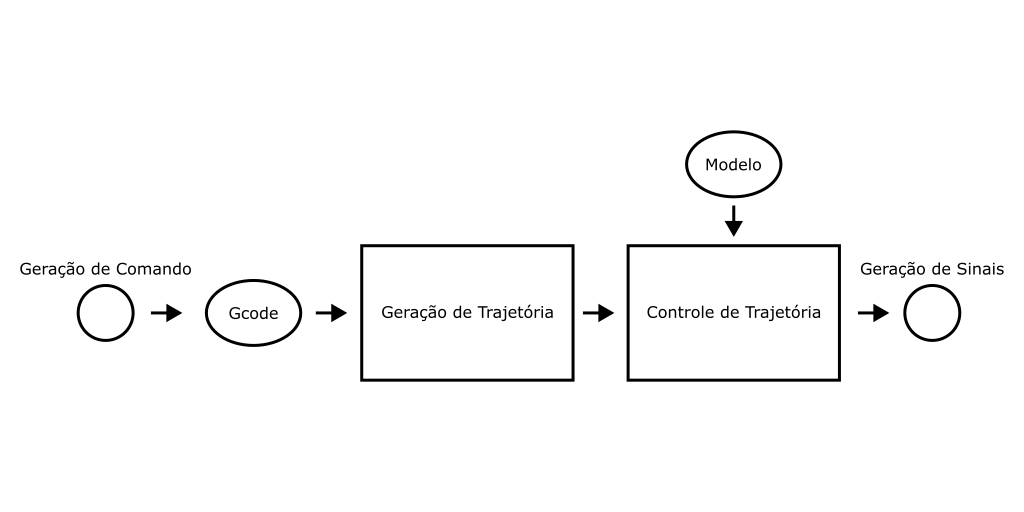
\includegraphics[scale=0.4]{fluxo_geral}

    \label{fig:fluxo_geral}
\end{figure}

\section{Geração de Trajetória}

A fase de geração de trajetória inicia-se com a análise do Gcode, que fornece as coordenadas e velocidades de destino dos movimentos. Neste processo, são considerados exclusivamente os comandos G1, que indicam movimentos lineares, e são extraídas as informações referentes aos eixos X, Y e à taxa de avanço (feedrate - F). É importante notar que a taxa de avanço, usualmente expressa em milímetros por minuto nos arquivos Gcode gerados por fatiadores, é convertida para milímetros por segundo.

\begin{figure}[H]
    \centering
    \caption{Curva de velocidade trapezoidal}
    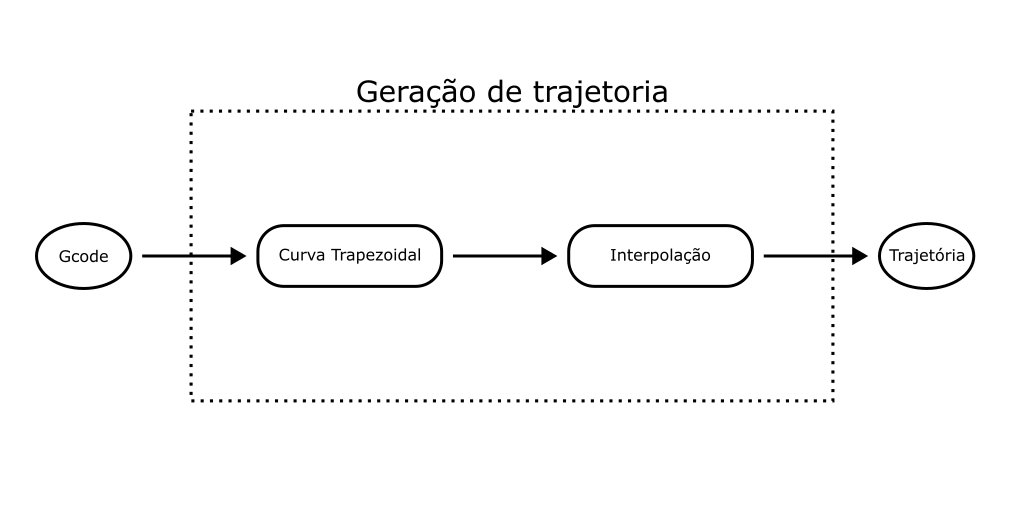
\includegraphics[scale=0.4]{geracao_de_trajetoria}

    \label{fig:geracao_de_trajetoria}
\end{figure}

\subsection{Curva trapezoidal de velocidade}

A próxima etapa  envolve a elaboração da curva trapezoidal de velocidade. Esta etapa se baseia em dados de entrada como deslocamento, velocidades iniciais e finais, e a velocidade almejada. A execução desta velocidade desejada é avaliada através do cálculo da velocidade de pico \(v_p\). Tal velocidade é obtida pela interseção das trajetórias de aceleração e desaceleração, que iniciam nas velocidades iniciais e finais respectivamente, e considerando que a área sob a curva deve ser equivalente ao deslocamento requerido. A fórmula para calcular \(v_p\) é expressa pela Equação \ref{eq:v_p}:

\begin{equation}
    \label{eq:v_p}
    v_p = \sqrt{\frac{(v_1^2+v_2^2)}{2}+a d}
\end{equation}

Nesta equação, \(v_1\) e \(v_2\) representam as velocidades iniciais e finais, \(a\) denota a aceleração definida na impressora, e \(d\) corresponde ao deslocamento.

A comparação entre a velocidade de pico e a velocidade desejada, esta última estabelecida pelo feedrate no Gcode, é crucial para definir se a trajetória do movimento adotará um perfil trapezoidal ou triangular de velocidade. A configuração do perfil depende da relação entre a velocidade de pico e a velocidade desejada: caso a primeira seja superior, o movimento será estruturado em três segmentos distintos, conforme ilustrado na Figura \ref{fig:trap_curv}.

\begin{figure}[H]
    \centering
    \caption{Curva de velocidade trapezoidal}
    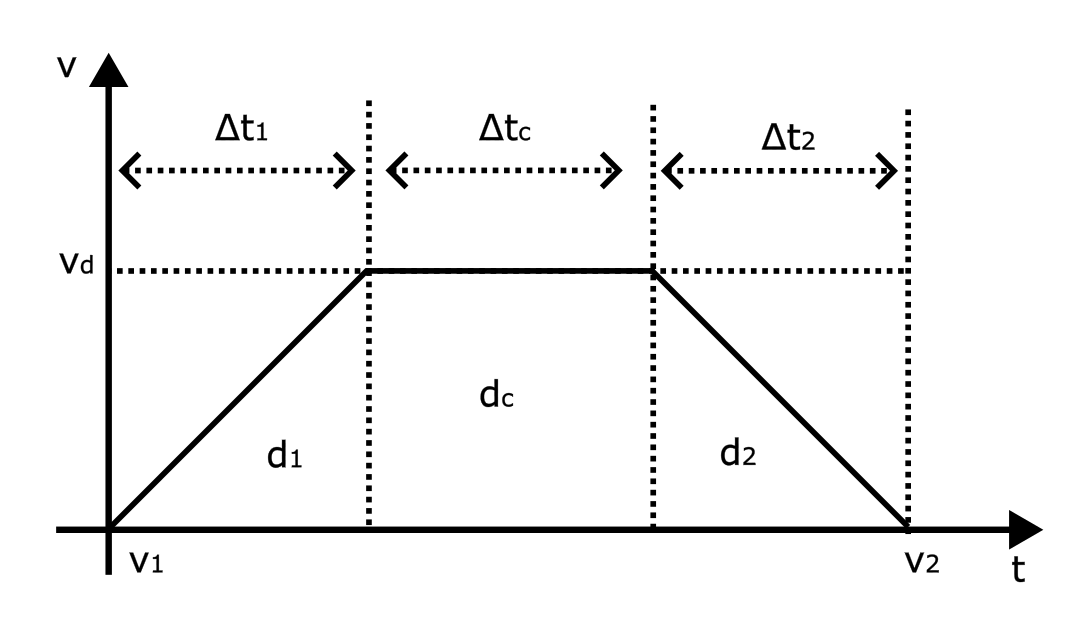
\includegraphics[scale=0.4]{trap_curv}
    \label{fig:trap_curv}
\end{figure}

Os segmentos de deslocamento \(d_1\), \(d_2\), e \(d_c\) correspondem às fases de aceleração, velocidade constante e desaceleração do movimento, respectivamente, e devem totalizar \(d\), o deslocamento total necessário. As variações temporais \(\Delta t_1\), \(\Delta t_2\), e \(\Delta t_c\) representam as durações de cada fase, baseadas nas velocidades inicial (\(v_1\)) e final (\(v_2\)), e na velocidade desejada (\(v_d\)). Os deslocamentos parciais são determinados pelas equações abaixo (Equação \ref{eq:des_seg_1_trap},  \ref{eq:des_seg_2_trap} e  \ref{eq:des_seg_c_trap}), que levam em conta a aceleração \(a\):

\begin{equation}
    \label{eq:des_seg_1_trap}
    d_1 = \frac{(v_d^2-v_1^2)}{(2 a)}
\end{equation}

\begin{equation}
    \label{eq:des_seg_2_trap}
    d_2 = \frac{(v_2^2-v_d^2)}{(2 a)}
\end{equation}

\begin{equation}
    \label{eq:des_seg_c_trap}
    d_c = d-(d_1+d_2)
\end{equation}

Os intervalos de tempo para as fases de aceleração, velocidade constante e desaceleração são calculados conforme (Equação \ref{eq:dt_seg_1_trap},  \ref{eq:dt_seg_2_trap} e  \ref{eq:dt_seg_c_trap}):

\begin{equation}
    \label{eq:dt_seg_1_trap}
    \Delta t_1 = \frac{(v_d-v_1)}{a}
\end{equation}

\begin{equation}
    \label{eq:dt_seg_2_trap}
    \Delta t_2 = \frac{(v_2-v_d)}{a}
\end{equation}

\begin{equation}
    \label{eq:dt_seg_c_trap}
    \Delta t_c = \frac{d_c}{v_d}
\end{equation}

Quando a velocidade de pico (\(v_p\)) é inferior à velocidade desejada (\(v_d\)), o perfil da trajetória de movimento assume uma forma triangular, em vez de trapezoidal. Esta condição implica que a velocidade desejada não é atingida durante o comando e, por conseguinte, o movimento é caracterizado por uma aceleração constante seguida de uma desaceleração constante, sem fase de velocidade constante. A Figura \ref{fig:triang_curv} ilustra este perfil de velocidade triangular.

\begin{figure}[H]
    \centering
    \caption{Curva de velocidade triangular}
    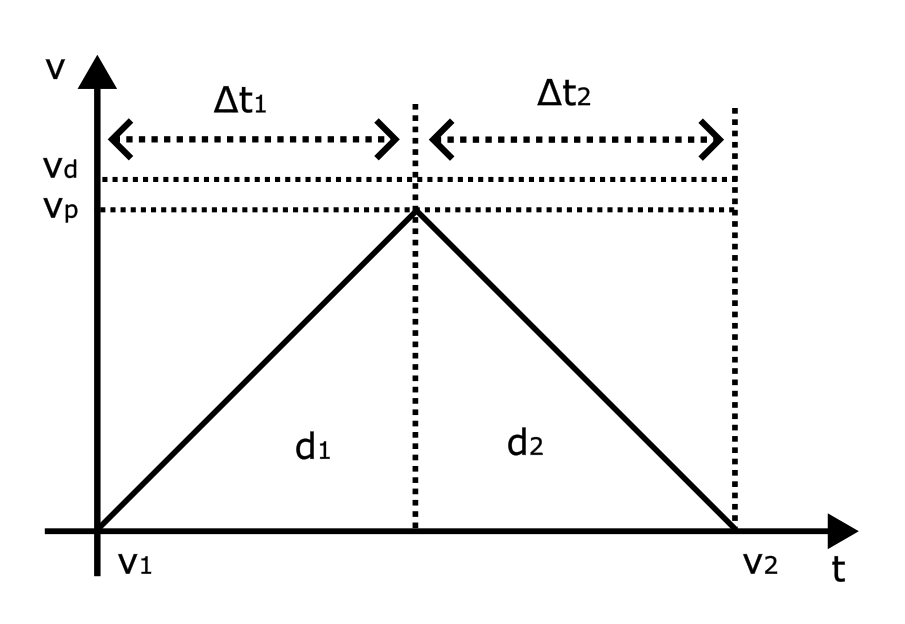
\includegraphics[scale=0.4]{triang_curv}

    \label{fig:triang_curv}
\end{figure}

Neste cenário, os segmentos de deslocamento \(d_1\) e \(d_2\) representam, respectivamente, as etapas de aceleração até a velocidade de pico e a desaceleração de volta à velocidade final. Os valores de \(d_1\) e \(d_2\) são calculados pelas seguintes equações (Equação \ref{eq:des_seg_1_tri}, \ref{eq:des_seg_2_tri}), que incorporam a aceleração (\(a\)) e as velocidades inicial (\(v_1\)) e final (\(v_2\)):

\begin{equation}
    \label{eq:des_seg_1_tri}
    d_1 = \frac{(v_p^2-v_1^2)}{(2 a)}
\end{equation}

\begin{equation}
    \label{eq:des_seg_2_tri}
    d_2 = \frac{(v_2^2-v_p^2)}{(2 a)}
\end{equation}

É possível calcular os intervalos de tempo dessas fases, através das Equações \ref{eq:dt_seg_1_tri} e \ref{eq:dt_seg_2_tri}.

\begin{equation}
    \label{eq:dt_seg_1_tri}
    t_1 = \frac{(v_p-v_1)}{a}
\end{equation}

\begin{equation}
    \label{eq:dt_seg_2_tri}
    t_2 = \frac{(v_2-v_p)}{a}
\end{equation}

Onde os tempos \(t_1\) e \(t_2\) representam, respectivamente, o tempo necessário para acelerar de \(v_1\) a \(v_p\) e para desacelerar de \(v_p\) a \(v_2\). 

Esses passos transformam a sequência de comandos movimentos do Gcode em uma trajetória com pontos com informações do deslocamento, velocidade, tempo, definidos nos nós onde ha alteração na aceleração, estabelecendo o comportamento dos movimentos de x e y no tempo.

\subsection{Interpolação}
A interpolação é um passo crucial para refinar a trajetória de movimento na impressão 3D. Esta fase trabalha sobre a trajetória definida para cada eixo na etapa anterior, empregando uma função de interpolação que gera pontos intermediários. Esses pontos são criados com base em um intervalo de tempo previamente definido, melhorando significativamente a resolução da trajetória.

Para subdividir esses intervalos de maneira eficaz, a Equação \ref{eq:N_steps} é utilizada para calcular o número de passos de interpolação necessários:

\begin{equation}
    \label{eq:N_steps}
    N = \lceil\frac{\Delta t}{\Delta p}-1\rceil
\end{equation}

Esta fórmula determina o número \( N \) de passos a serem tomados dentro de um dado intervalo de tempo \( \Delta t \), com cada passo tendo um período \( \Delta p \). Após a divisão dos intervalos, a Equação \ref{eq:dt_interpol_last_step} calcula o tempo restante no último passo de interpolação (\(\Delta t_f\)):

\begin{equation}
    \label{eq:dt_interpol_last_step}
    \Delta t_f= \Delta t - \Delta p N 
\end{equation}

Finalmente, com base nesses passos de tempo determinados (\(\Delta t_i\)) anexando \(\Delta t_f\) à lista de passos \(\Delta p\) de tamanho \(N\), a Equação \ref{eq:delta_des_interpol} é empregada para calcular o deslocamento correspondente a cada passo (\(\Delta d_i\)), utilizando a aceleração do segmento a ser interpolado (\(a_s\)) e a velocidade inicial do segmento (\(v_s\)):

\begin{equation}
    \label{eq:delta_des_interpol}
    \Delta d_i = \Delta v_s \Delta t_i+ \frac{a_s \Delta t_i^2}{2} 
\end{equation}

Esses cálculos são fundamentais para garantir que a trajetória seja suficientemente detalhada, permitindo que a fase de controle da trajetória seja executada com sucesso.

\section{Modelagem dinâmica de uma impressora 3D}

A modelagem do sistema mecânico da impressora 3D é um passo crucial para a implementação eficaz do método proposto. Essa modelagem não só facilita a compreensão do comportamento da impressora mas também é fundamental para definir as restrições necessárias na etapa subsequente de controle de trajetória, restrições essas que aplicam as equações de movimento e condições de contorno definidas no modelo.

É fundamental enfatizar a importância de um modelo representativo. A eficácia do método proposto depende diretamente da acurácia com que o modelo simula o comportamento real da impressora 3D. Neste estudo, consideramos as seguintes características principais do sistema:

\begin{itemize}
    \item Influência da Correia: A correia é o componente chave responsável por introduzir desvios nas trajetórias de impressão. Ela age como uma combinação de mola e amortecedor, afetando a dinâmica do movimento.
    \item Modelagem do Conjunto Bico Injetor e Extrusora: Este conjunto é tratado como um corpo rígido uniforme, simplificando sua representação geométrica. Sua massa é considerada como 200g, o que influencia a dinâmica do movimento.
    \item Dimensões da Mesa de Impressão: A área útil da mesa de impressão é de 200 mm x 200 mm, definindo o espaço de trabalho disponível.
    \item Configuração Cartesiana: A impressora opera em um sistema cartesiano, com eixos ortogonais, o que simplifica a análise de movimento.
    \item Independência dos Eixos: Cada eixo da impressora opera independentemente dos outros, permitindo uma análise mais simplificada das dinâmicas individuais.
    \item Condições Iniciais de Movimento: Assume-se que todos os movimentos da impressora iniciam a partir do estado de repouso.
\end{itemize}

Com base nesses parâmetros, definimos duas posições-chave para análise em cada eixo. A primeira é a posição ideal (\(x_b\)) ou posição da base, que representa o ponto desejado pelo usuário, assumindo um sistema sem flexibilidade ou perdas. A segunda é a posição real (\(x_p\)) ou a posição da ponta, que leva em conta as forças inerciais e a flexibilidade introduzida pela correia. Este modelo é ilustrado na figura \ref{fig:model_1_axis}.

\begin{figure}[H]
    \centering
    \caption{Modelagem de 1 eixo}
    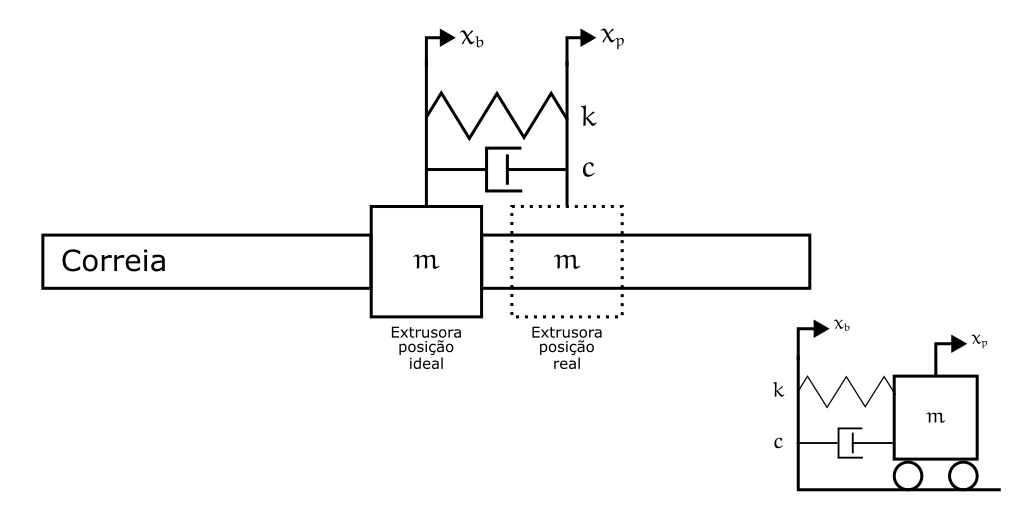
\includegraphics[scale=0.4]{model_1_axis}

    \label{fig:model_1_axis}
\end{figure}

As equações de movimento para a impressora são descritas a seguir:
\begin{multline}
    \label{eq:mov_impressora}
    \\
    m \ddot{x_p} + c(\dot{x_p} - \dot{x_b}) + k(x_p-x_b) = 0 \\
    \ddot{x_p} = - \frac{c}{m} \dot{x_p} - \frac{k}{m} x_p + \frac{c}{m} \dot{x_b} + \frac{k}{m} x_b \\
\end{multline}

Nestas equações, \(m\) representa a massa do conjunto bico injetor e extrusora, \(c\) é a constante de amortecimento da correia, e \(k\) é a constante da mola equivalente da correia. As variáveis \(x_p\) e \(x_b\) correspondem, respectivamente, às posições da ponta e da base do componente em movimento. Essas equações fundamentam o modelo dinâmico que empregamos para simular e otimizar a trajetória de impressão na impressora 3D. Na Figura \ref{fig:model_2_axis} é representada a composição dos eixos x e y utilizado neste estudo, sendo considerada a aplicação das Equação \ref{eq:mov_impressora} para cada um dos eixos de maneira análoga, podendo identificar o eixo através dos subindices \(x\) e \(y\), ou no caso das posições o eixo y é identificado por \(y_p\) e \(y_b\) (posição da ponta do eixo y e posição da base do eixo y respectivamente).

\begin{figure}[H]
    \centering
    \caption{Modelagem dos eixos x e y}
    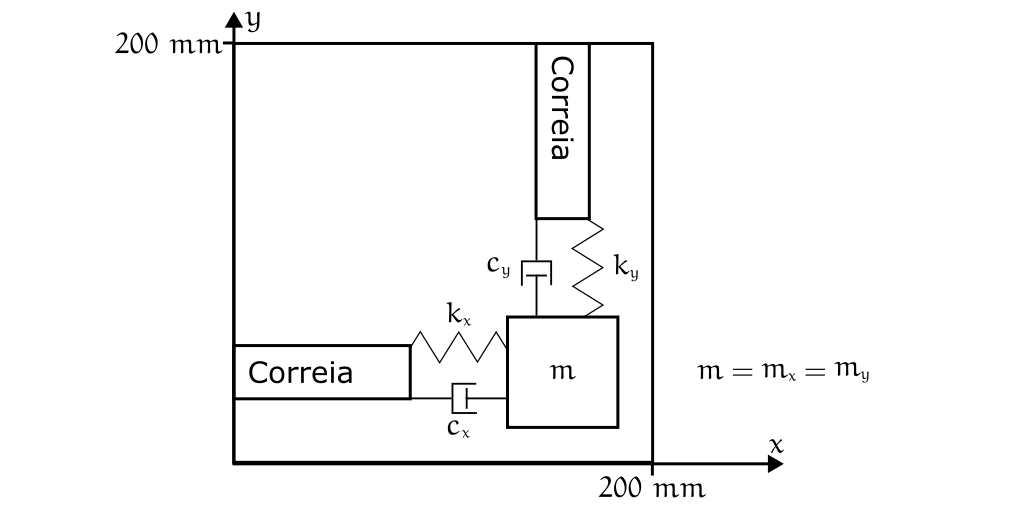
\includegraphics[scale=0.4]{model_2_axis}

    \label{fig:model_2_axis}
\end{figure}

\subsection{Espaço de estados}
A formulação do espaço de estados é adotada neste estudo para simplificar as operações e a solução do sistema dinâmico da impressora 3D. Esta abordagem é eficaz pois transforma uma equação diferencial de ordem superior em um sistema de equações diferenciais de primeira ordem, mas com um número maior de equações. Esta metodologia facilita o entendimento e a manipulação das dinâmicas do sistema.

O modelo dinâmico no espaço de estados é representado na seguinte forma (Equação \ref{eq:simp_state_space_din_model}):

\begin{equation}
    \label{eq:simp_state_space_din_model}
    \dot x = A*x+B*u
\end{equation}

Nesta equação, \(\dot x\) representa o vetor de estados derivados, \(x\) é o vetor de estados, \(A\) é a matriz do sistema que define a relação entre os estados atuais e suas taxas de mudança, \(u\) é o vetor de entradas externas, e \(B\) é a matriz de controle que relaciona as entradas com os estados.

Baseado na equação de movimento \ref{eq:mov_impressora}, análogos ao eixo y, expandimos as matrizes e vetores para representar com precisão a dinâmica do sistema no espaço de estados, conforme apresentado na equação \ref{eq:espaco_de_estados_din_model}:

\begin{equation}
    \label{eq:espaco_de_estados_din_model}
    \begin{bmatrix}
        \dot{x_p} \\
        \ddot{x_p} \\
        \dot{y_p} \\
        \ddot{y_p}
    \end{bmatrix}
    =
    \begin{bmatrix}
        0 & 1 & 0 & 0 \\
        -\frac{k_x}{m_x} & -\frac{c_x}{m_x} & 0 & 0 \\
        0 & 0 & 0 & 1 \\
        0 & 0 & -\frac{k_x}{m_x} & -\frac{c_x}{m_x}
    \end{bmatrix}
    \begin{bmatrix}
        x_p \\
        \dot{x_p} \\        
        y_p \\
        \dot{y_p} \\
    \end{bmatrix}
    +
    \begin{bmatrix}
        0 & 0 & 0 & 0 \\
        \frac{k_x}{m_x} & \frac{c_x}{m_x} & 0 & 0 \\
        0 & 0 & 0 & 0 \\
        0 & 0 & \frac{k_x}{m_x} & \frac{c_x}{m_x}
    \end{bmatrix}
    \begin{bmatrix}
        x_b \\
        \dot{x_b}  \\
        y_b \\
        \dot{y_b} 
    \end{bmatrix}
\end{equation}

Nesta equação, \(x_p\) e \(y_p\) são as posições reais (da ponta) nos eixos X e Y, respectivamente, enquanto \(x_b\) e \(y_b\) são as posições ideais (da base). As variáveis \(\dot{x_p}\) e \(\dot{y_p}\) representam a primeira derivada do tempo das posições nos eixos X e Y, indicando a velocidade e aceleração. \(k_x\) e \(k_y\) denotam as constantes elásticas das correias nos eixos X e Y, enquanto \(c_x\) e \(c_y\) representam as constantes de amortecimento dessas correias. \(m_x\) e \(m_y\) são as massas associadas aos conjuntos de bico injetor e extrusora nos respectivos eixos.

\section{Controle de Trajetória}

\begin{figure}[H]
    \centering
    \caption{Fluxograma Controle de Trajetória}
    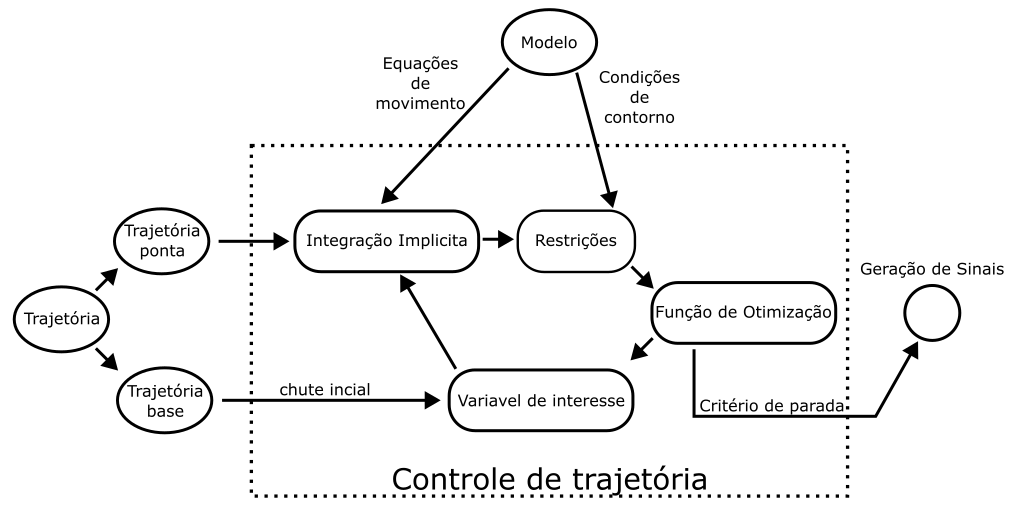
\includegraphics[scale=0.4]{controle_de_trajetoria}

    \label{fig:controle_de_trajetoria}
\end{figure}

\subsection{Integração Implícita}
\subsection{Variável de interesse}
\subsection{Restrições}
\subsection{Função de Otimização (Minimização)}

\subsection{Restrições lineares e limites de borda}

Não foram utilizadas restrições lineares na otimização. Os limites superiores (\textit{upperbound}) e inferiores (\textit{lowerbound}) foram definidos com base nos limites físicos da impressora para as posições $x_b$ e $y_b$ (ver Seção \ref{parametrosimp}).

\subsection{Restrições não lineares}

A função para as restrições não lineares foi implementada com base nas equações \ref{eq:state_center_segment}, \ref{eq:state_dot_center_segment}, \ref{eq:defect_calc}, \ref{eq:input_value_center_segment} de maneira a popular a variável de restrições de igualdades com os valores do defeito dos segmentos ($\Delta$) e também com os valores iniciais. 

A arrancada também foi utilizada como restrição de equalidade, atrelada ao condicional ?? para que se comporte como uma inequalidade. A variável de restrições de inequalidades não foi populada (ver Seção ?? Resultados e Discussão).

% \subsection{Função objetivo}

% Foram realizados alguns testes com funções objetivo e seus resultados são apresentados na seção de resultados e discussão,
% entretanto a função objetiva foi definida como zero, ou seja, pra qualquer valor ela retornara zero nas chamadas da FMINCON.

\subsection{Solução da trajetória da base}

É considerada como trajetória desejada a trajetória obtida através da função de geração de comando apresentada anteriormente e são utilizados os vetores de tempo e posição como variáveis globais, para serem acessados dentro da função das restrições não lineares, chamada pela FMINCON. Além disso, esses mesmos vetores de posição também são considerados como o chute inicial e variável principal
na FMINCON, sendo adaptados em forma de matriz.

A variável principal inserida na FMINCON é a matriz contendo os vetores de posição da base ($x_b$ e $y_b$), enquanto os vetores de posição da ponta são fixados pela trajetória desejada presente na forma de variáveis globais.

As Equações \ref{eq:der_a} e \ref{eq:der_b} foram utilizadas para reconstrução do vetor de velocidade a partir dos vetores deslocamento e tempo, sendo $dt$ a variação do tempo no intervalo, $des_n$ o deslocamento final do intervalo, $des_i$ o deslocamento inicial no intervalo, $a_n$ a aceleração do intervalo, $v_n$ a velocidade final do intervalo e $v_i$ a velocidade inicial do intervalo. 

% Para conseguir realizar os cálculos necessários dentro da função de restrições não lineares é utilizado o seguinte conjunto
% de equações basicas (\ref{eq:der_a}) para se derivar a curva posição-tempo considerando aceleração constante,
% sendo $dt$ a variação do tempo no intervalo, $des_n$ o deslocamento final do intervalo, $des_i$ o deslocamento inicial no intervalo,
% $a_n$ a aceleração do intervalo, $v_n$ a velocidade final do intervalo e $v_i$ a velocidade inicial do intervalo.
% Assim construindo o vetor de velocidade a partir da condição inicial de deslocamento e velocidade zero, para ambos os eixos ($x$ e $y$).

\begin{equation}
    \label{eq:der_a}      
        a(k) = \frac{2}{\Delta t(k)} \left( \frac{d(k)-d(k-1)}{\Delta t(k)}-v(k-1) \right)
\end{equation}

\begin{equation}
    \label{eq:der_b}      
        v(k) = v(k-1)+a(k) \Delta t(k)
\end{equation}

\subsection{Configurações da função}

A Tabela \ref{tab:fmincon_options} apresenta o conjunto de configurações customizadas da função FMINCON. As configurações não explicitadas foram mantidas como os padrões disponibilizados pelo Matlab. A função objetivo foi considerada nula por hipótese.

\begin{table}
    \begin{center}
    \caption{Parâmetros modificados na função FMINCON.}
    \label{tab:fmincon_options}
    \begin{tabular}{c c}
        Opção & Valor \\ \hline
        TolFun & 0.000000001 \\
        MaxIter & 100000 \\
        Display & iter \\
        DiffMinChange & 0.0001 \\
        Algorithm & interior-point \\
        StepTolerance & 1e-12 \\
        MaxFunEvals & 700000  \\ \hline
    \end{tabular}
    \end{center}
\end{table}

\section{Simulação Computacional e Análise de Dados}

\subsection{Caso base} 

Com base no modelo proposto, foi simulada a trajetória do ponteiro em 10 milímetros ao longo do eixo x e depois 10 milímetros ao longo do eixo y. Para as análises do caso base, foram avaliados os cenários com controle e sem controle. Também foram analisados os perfis de deslocamento e velocidade. 

A Tabela \ref{tab:base_params} apresenta os parâmetros de frequência, coeficiente de amortecimento, aceleração base, velocidade desejada e resolução de interpolação ("parâmetros-chave") considerados para este cenário base.

\begin{table}
    \begin{center}
    \caption{Parâmetros referência dos Estudos de Caso.}
    \label{tab:base_params}
    \begin{tabular}{c c c}
        Parâmetro & Valor & Unidade\\ \hline
        Frequência & 100 & $rad/s$\\
        Coeficiente de amortecimento & 0,5 & - \\
        Aceleração base & 5000 & $mm/s^2$ \\
        Velocidade desejada & 100 & $mm/s$ \\
        Resolução de interpolação & 0,005 & $s$ \\ \hline
    \end{tabular}
    \end{center}
\end{table}

\subsection{Análise de sensibilidade}

O tamanho dos vetores, o tempo de simulação e o índice viabilidade da FMINCON também foram analisados. O tamanho dos vetores é definido na fase de geração de comando e tem influência direta da resolução de interpolação definida e do tempo necessário para percorrer o caminho dada as definições de velocidades na geração de comando. O tempo de simulação começa a ser contado logo depois da geração de comando e para quando a função FMINCON termina de ser executada. A viabilidade é um dos resultados da função FMINCON e este representa o valor da maior restrição não cumprida.

\begin{figure}[H]
    \centering
    \caption{Curva de velocidade trapezoidal}
    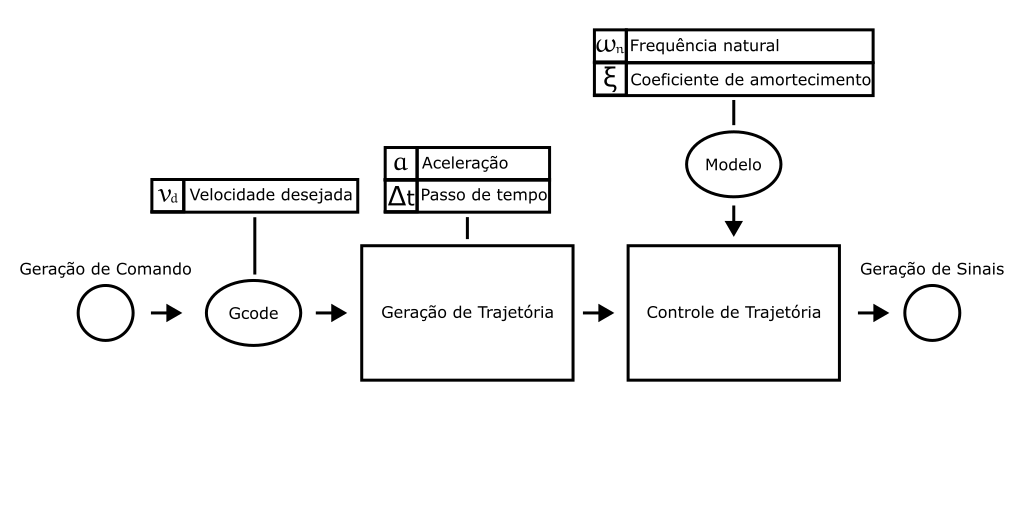
\includegraphics[scale=0.4]{fluxo_geral_var}

    \label{fig:fluxo_geral_var}
\end{figure}

O computador utilizado para a realização das simulações foi um notebook Acer com as configurações apresentadas na Tabela
\ref{tab:note_config}.

\begin{table}
    \begin{center}
    \caption{Estudos de Caso}
    \label{tab:sim_params}
    \begin{tabular}{c c c c c c}
        Caso & Parâmetro & Valor A & Valor B & Valor C & Unidade\\ \hline
        1 & Frequência & 50 & 200 & 500 & $rad/s$\\
        2 & Coeficiente de amortecimento & 0 & 1 & 2 & - \\
        3 & Aceleração base & 1000 & 10000 & - & $mm/s^2$ \\
        4 & Velocidade desejada & 50 & 200 & - & $mm/s$ \\
        5 & Resolução de interpolação & 0,01 & 0,001 & 0,0002 & $s$ \\ \hline
    \end{tabular}
    \end{center}
\end{table}


Além das curvas de posição, deslocamento e velocidade, algumas variáveis também foram explicitadas para análise. São elas o tamanho dos vetores, o tempo de simulação e a viabilidade ao longo. O tamanho dos vetores é definido na fase de geração de comando e tem influência direta da resolução de interpolação definida e do tempo necessário para percorrer o caminho dada as definições de velocidades na geração de comando. O tempo de simulação começa a ser contado logo depois da geração de comando e para quando a função FMINCON termina de ser executada. A viabilidade é um dos resultados da função FMINCON e este representa o valor da maior restrição não cumprida.

A máquina utilizada para a realização das simulações foi um notebook acer com as configurações apresentadas na tabela
\ref{tab:note_config}.

\begin{table}
    \begin{center}
    \caption{Especificações do computador}
    \label{tab:note_config}
    \begin{tabular}{c c}
        \hline
        Processador & Intel I7-5500U 2.40GHz \\
        Memoria & 8,00 GB \\
        Placa de vídeo & Nvidia Geforce 920M \\
        Sistema & 64 bits \\ \hline
    \end{tabular}
    \end{center}
\end{table}
